As telas a seguir foram capturadas com o arquivo .pkt entregue aberto no Cisco Packet Tracer 9.0.1, depois de reiniciar o cenário com o botão de \emph{power cycle}. Como a startup-config de todos os equipamentos é igual à running-config, nada se perdeu no reinício. Cada tela corresponde a um teste da seção 4. As imagens em tamanho original estão no repositório do trabalho, em \url{https://github.com/gabrielandre-math/Trabalho-de-Redes-I---UERJ}.

\subsecao{B.1 Cenário}

Depois do reinício e da convergência do spanning tree, todos os enlaces ficam verdes. As notas ao lado dos PCs trazem a VLAN, a subrede, a máscara e o gateway, como o roteiro pede.

\begin{figure}[H]
\captionsetup{position=top}
\caption{cenário no Packet Tracer com as notas de endereçamento}\label{fig:print-topo}
\centering
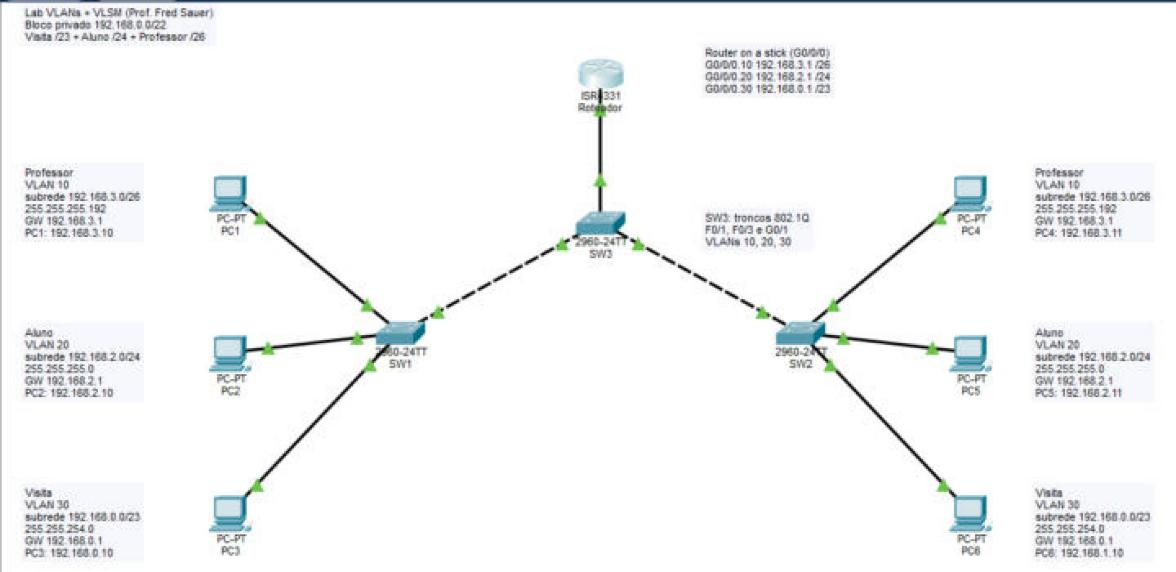
\includegraphics[width=\textwidth]{prints/topologia.png}
\fonteprint
\end{figure}

\subsecao{B.2 Switches}

Nos três switches o \texttt{show vlan brief} lista as VLANs 10 (professor), 20 (aluno) e 30 (visita). No SW1 e no SW2 as portas Fa0/11, Fa0/18 e Fa0/6 aparecem nas suas VLANs, e o \texttt{show interfaces trunk} mostra um tronco em cada um (Fa0/1 no SW1 e Fa0/3 no SW2). No SW3 as VLANs existem sem portas de acesso e os três troncos (Fa0/1, Fa0/3 e Gig0/1) aparecem em modo \emph{on}, com encapsulamento 802.1q, VLAN nativa 1 e somente as VLANs 10, 20 e 30 permitidas.

\begin{figure}[H]
\captionsetup{position=top}
\caption{SW1: show vlan brief e show interfaces trunk}\label{fig:print-sw1}
\centering
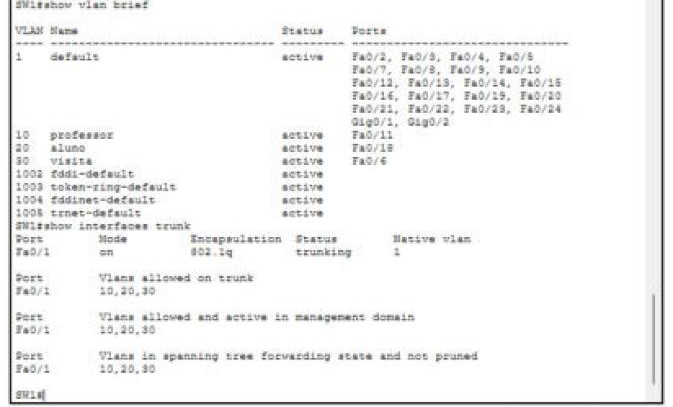
\includegraphics[width=0.70\textwidth]{prints/sw1.png}
\fonteprint
\end{figure}

\begin{figure}[H]
\captionsetup{position=top}
\caption{SW2: show vlan brief e show interfaces trunk}\label{fig:print-sw2}
\centering
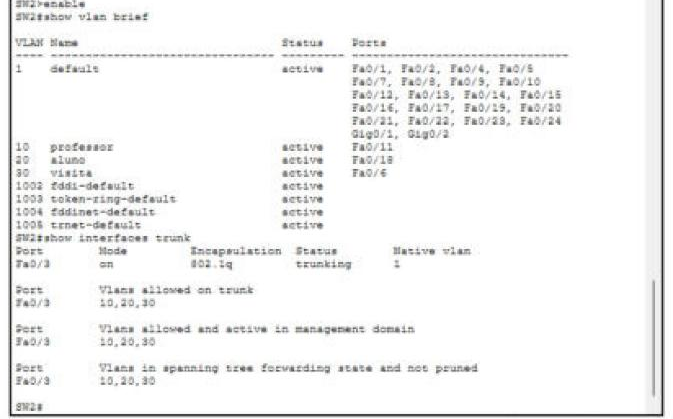
\includegraphics[width=0.70\textwidth]{prints/sw2.png}
\fonteprint
\end{figure}

\begin{figure}[H]
\captionsetup{position=top}
\caption{SW3: show vlan brief e show interfaces trunk}\label{fig:print-sw3}
\centering
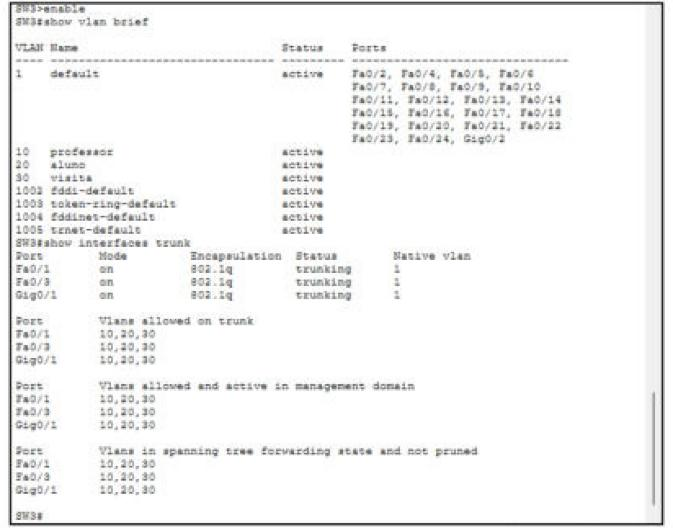
\includegraphics[width=0.70\textwidth]{prints/sw3.png}
\fonteprint
\end{figure}

\subsecao{B.3 Roteador}

O \texttt{show ip interface brief} mostra a G0/0/0 e as três subinterfaces \emph{up/up}, com os IPs dos gateways. O \texttt{show ip route} mostra as três redes diretamente conectadas (192.168.0.0/23, 192.168.2.0/24 e 192.168.3.0/26), cada uma na sua subinterface.

\begin{figure}[H]
\captionsetup{position=top}
\caption{roteador: show ip interface brief e show ip route}\label{fig:print-rot}
\centering
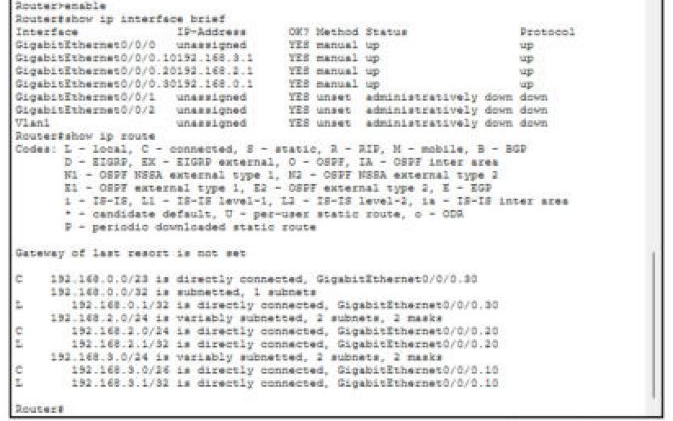
\includegraphics[width=0.78\textwidth]{prints/roteador.png}
\fonteprint
\end{figure}

\subsecao{B.4 Ping e tracert nos PCs}

No PC1 (VLAN 10), o ping para o PC4 (192.168.3.11, mesma VLAN) responde com TTL=128 e o ping para o PC5 (192.168.2.11, VLAN 20) responde com TTL=127, porque passou uma vez pelo roteador. O tracert para o PC5 mostra os dois saltos: o gateway 192.168.3.1 e o destino.

\begin{figure}[H]
\captionsetup{position=top}
\caption{PC1: ping para o PC4, ping para o PC5 e tracert para o PC5}\label{fig:print-pc1}
\centering
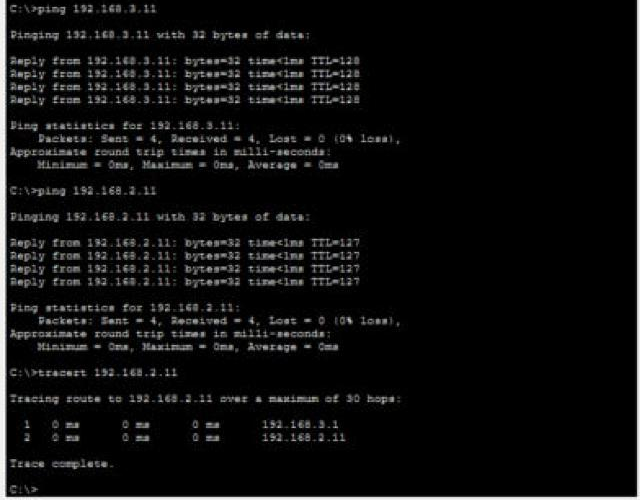
\includegraphics[width=0.62\textwidth]{prints/pc1.png}
\fonteprint
\end{figure}

No PC3 (VLAN 30, 192.168.0.10/23), o tracert para o PC6 (192.168.1.10) tem um salto só, sem passar pelo roteador, embora o 3º octeto seja diferente: os dois estão na mesma /23. O ping para o PC1, que está em outra VLAN, responde com TTL=127.

\begin{figure}[H]
\captionsetup{position=top}
\caption{PC3: ipconfig, tracert para o PC6 e ping para o PC1}\label{fig:print-pc3}
\centering
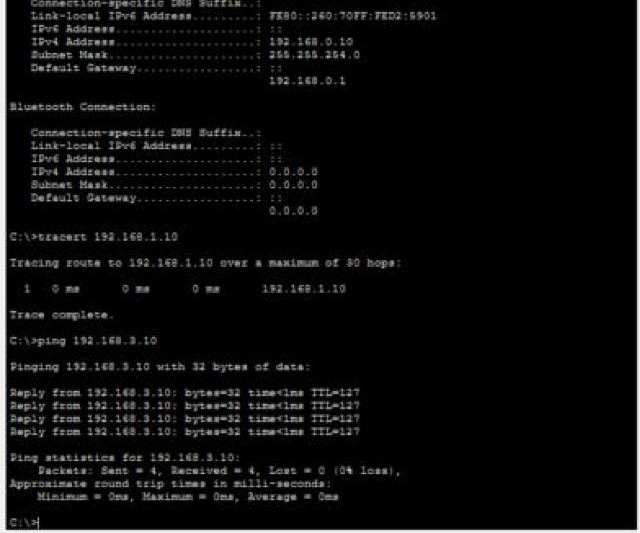
\includegraphics[width=0.62\textwidth]{prints/pc3.png}
\fonteprint
\end{figure}

No PC6 (VLAN 30, 192.168.1.10/23), o tracert para o PC2 (192.168.2.10) passa pelo gateway 192.168.0.1 e chega ao destino. O asterisco na primeira medida do segundo salto é o pacote descartado enquanto o roteador resolvia o MAC do PC2 por ARP. O ping para o próprio gateway responde com TTL=255, o TTL inicial do roteador.

\begin{figure}[H]
\captionsetup{position=top}
\caption{PC6: ipconfig, tracert para o PC2 e ping para o gateway}\label{fig:print-pc6}
\centering
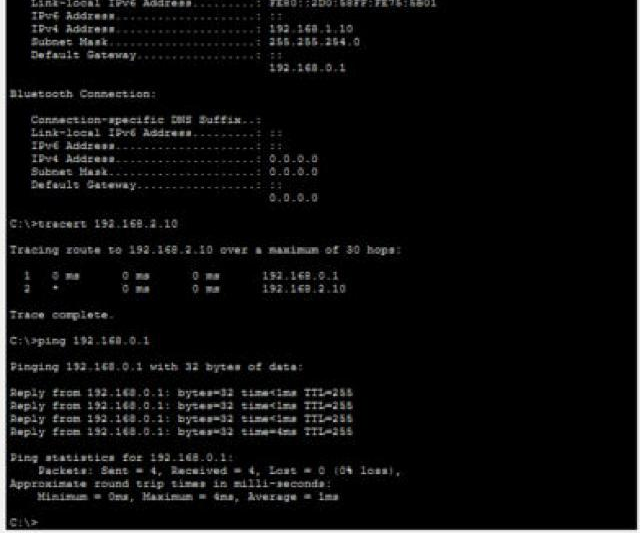
\includegraphics[width=0.62\textwidth]{prints/pc6.png}
\fonteprint
\end{figure}

\subsecao{B.5 Modo simulação}

Com o cenário recém-reiniciado e o filtro em ARP e ICMP, fiz o ping do PC1 para o PC5 no modo simulação. A Figura~\ref{fig:print-sim1} mostra o início da lista de eventos. O broadcast ARP do PC1 passa por SW1, SW3 e SW2 e chega somente ao PC4 e ao roteador, que são os equipamentos da VLAN 10. O primeiro \emph{echo request} vai até o roteador, que então envia o seu ARP na VLAN 20, recebido somente pelo PC2 e pelo PC5.

\begin{figure}[H]
\captionsetup{position=top}
\caption{lista de eventos: ARP do PC1 na VLAN 10 e ARP do roteador na VLAN 20}\label{fig:print-sim1}
\centering
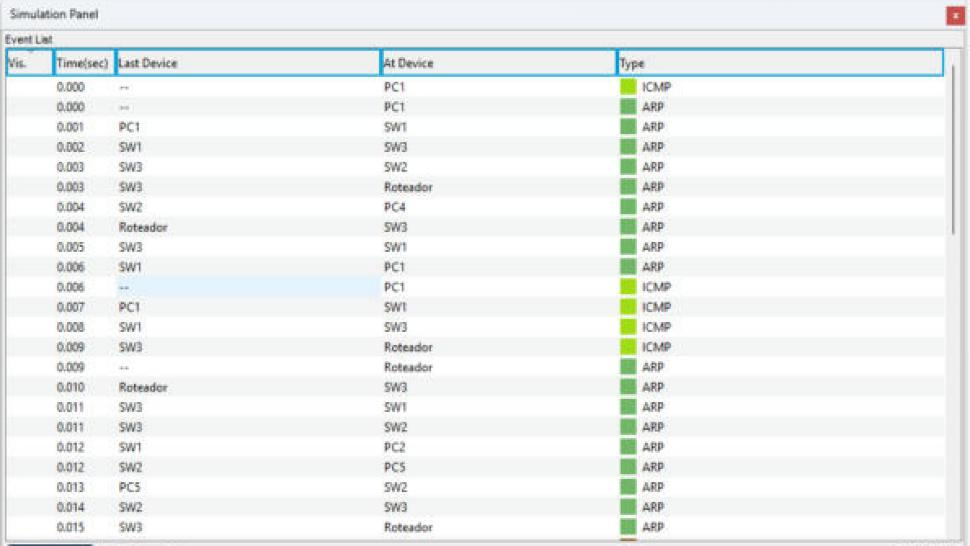
\includegraphics[width=0.88\textwidth]{prints/sim1.png}
\fonteprint
\end{figure}

A Figura~\ref{fig:print-sim2} mostra o segundo ping completo: PC1, SW1, SW3, roteador, SW3, SW2 e PC5 na ida, e o caminho inverso na volta. O pacote passa duas vezes pelo enlace entre o SW3 e o roteador, que é o comportamento do \emph{router on a stick}. Ao fim dos quatro pings o Packet Tracer avisou que o buffer de eventos estava cheio, como o roteiro previa.

\begin{figure}[H]
\captionsetup{position=top}
\caption{lista de eventos: echo request e echo reply passando pelo roteador}\label{fig:print-sim2}
\centering
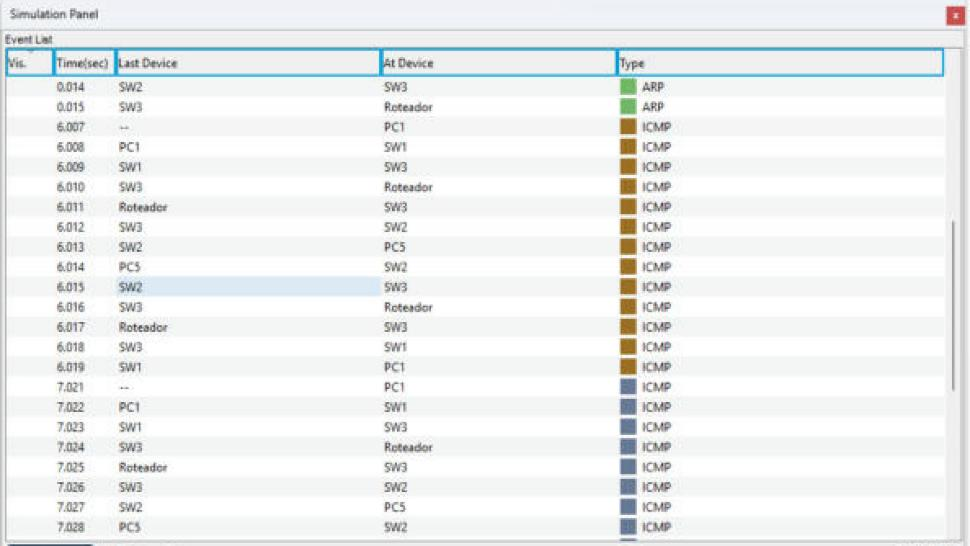
\includegraphics[width=0.88\textwidth]{prints/sim2.png}
\fonteprint
\end{figure}
